\documentclass{article}
\usepackage{ctex}
\usepackage{graphicx}
\usepackage{amsmath}
\usepackage{indentfirst}
\usepackage{titlesec}
\usepackage{setspace}
\usepackage{subfigure}
\usepackage{caption}
\usepackage{float}
\usepackage{booktabs}
\usepackage{geometry}
\usepackage{multirow}
\usepackage{hyperref}
\hypersetup{
	colorlinks=true,
	linkcolor=blue,
	filecolor=magenta,      
	urlcolor=cyan,
	pdftitle={Overleaf Example},
	pdfpagemode=FullScreen,
}
\geometry{left=1.2cm,right=1.2cm,top=2cm,bottom=2cm}
\title{\songti \zihao{2}\bfseries HW11第17题DLA分形维数}
\titleformat*{\section}{\songti\zihao{4}\bfseries}
\titleformat*{\subsection}{\songti\zihao{5}\bfseries}
\renewcommand\thesection{\arabic{section}}
\author{王启骅 PB20020580}
\begin{document}
	\maketitle
	\section{题目}
进行单中心DLA模型的模拟(可以用圆形边界,也可
以用正方形边界),并用两种方法计算模拟得到的DLA图形的分
形维数,求分形维数时需要作出双对数图。
	\section{算法原理}
	首先使用DLA方法产生生长模型,生长方法如下。运用2维DLA模型,首先生成一个二维$ L\times L=1001\times1001 $的mesh网格,用1作为生长点,0作为未生长的点。在网格中心$ (\frac{L+1}{2},\frac{L+1}{2}) $放置结晶核设置为1。
	
	
	在模拟的每次记录新结晶点到原点的距离,与当前最大半径进行比对,得到当前图形的最大半径$ r_{max} $。n为已产生的粒子数。则在这里在半径为$ start=r_{max}+\delta r $的圆上,通过生成$ [0,2\pi] $均匀分布的随机数生成在圆上均匀产生的粒子。设定在粒子游走到$ edge=2*(r_{max}+\delta r) $的圆外时认为消失,进行下一次模拟。当edge达到mesh网格的边界处时,即$2*(r_{max}+\delta r)>\frac{L-1}{2}-1 $时,直接设定$ edge=\frac{L-1}{2}-1 $。如果游走到周围有格点为1时,则将该粒子所在的格点设为1,认为生长,并进行下一次模拟。
	
	
	接下来计算图形的分形维数,一下使用两种方法。
	
	
	首先使用sandbox法,在已经生成好的图形中,使用边长为$ r=2*i $的正方形网格,以$ (\frac{L+1}{2},\frac{L+1}{2}) $为中心,记录网格中的像素数N,对结果$ \ln N\sim \ln r $线性拟合得到的斜率即为分形维数D。
	
	
	接下来使用面积-回转半径法。这里可以对于生长过程中的各个时间的单个结晶结果认为是多个结晶生长的平均,从而将该方法推广至单个生长的情况。对于每个新生长的质点,计算构型的回转半径
	\begin{equation}
		R_g^2=\frac{\sum r_i^2}{N}
	\end{equation}
	之后线性拟合$ \ln N\sim \ln R_g $得到斜率即为该分形维数。
	
	\section{结果}
\subsection{DLA结果}
以下是DLA生长在n=$ 100,10^3,10^4,10^5 $下的结果。如图\ref{fig:1}
 \begin{figure}[!h]
	\centering
	\subfigure[$ n=100 $]{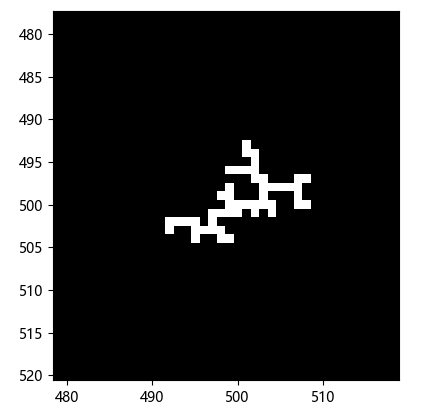
\includegraphics[scale=0.6]{mesh_2}}
	\subfigure[$ n=10^3 $]{	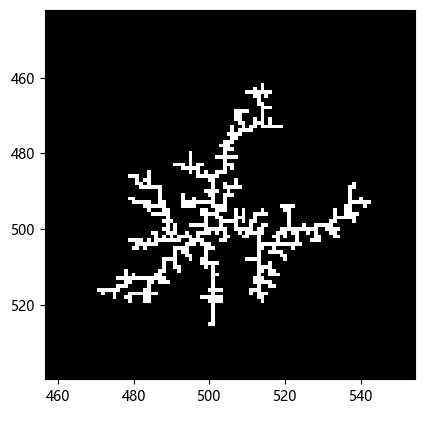
\includegraphics[scale=0.6]{mesh_3}}
	
	\subfigure[n=$ 10^4 $]{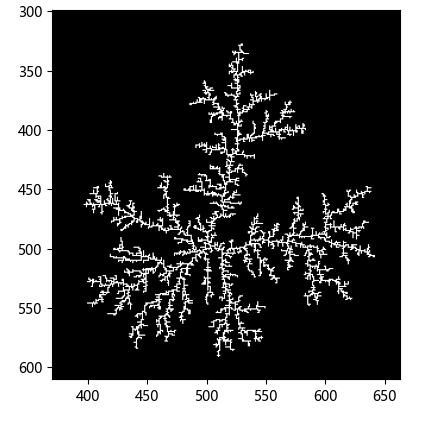
\includegraphics[scale=0.6]{mesh_4}}
	\subfigure[n=$ 10^5 $]{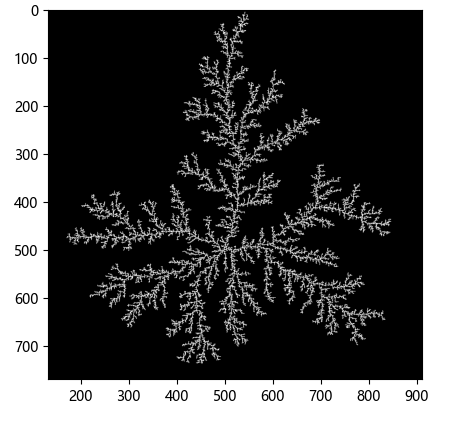
\includegraphics[scale=0.6]{mesh_5}}
	\captionsetup{font={small},labelfont=bf}
	\caption{\heiti\zihao{-5}DLA生长结果}
	\label{fig:1}
\end{figure}
\subsection{Sandbox计数法}
这里采用正方形边长为$ r=2-2^9 $进行计数。计算得到的拟合曲线如图\ref{fig:2}
		\begin{figure}[!h]
	
	\centering
	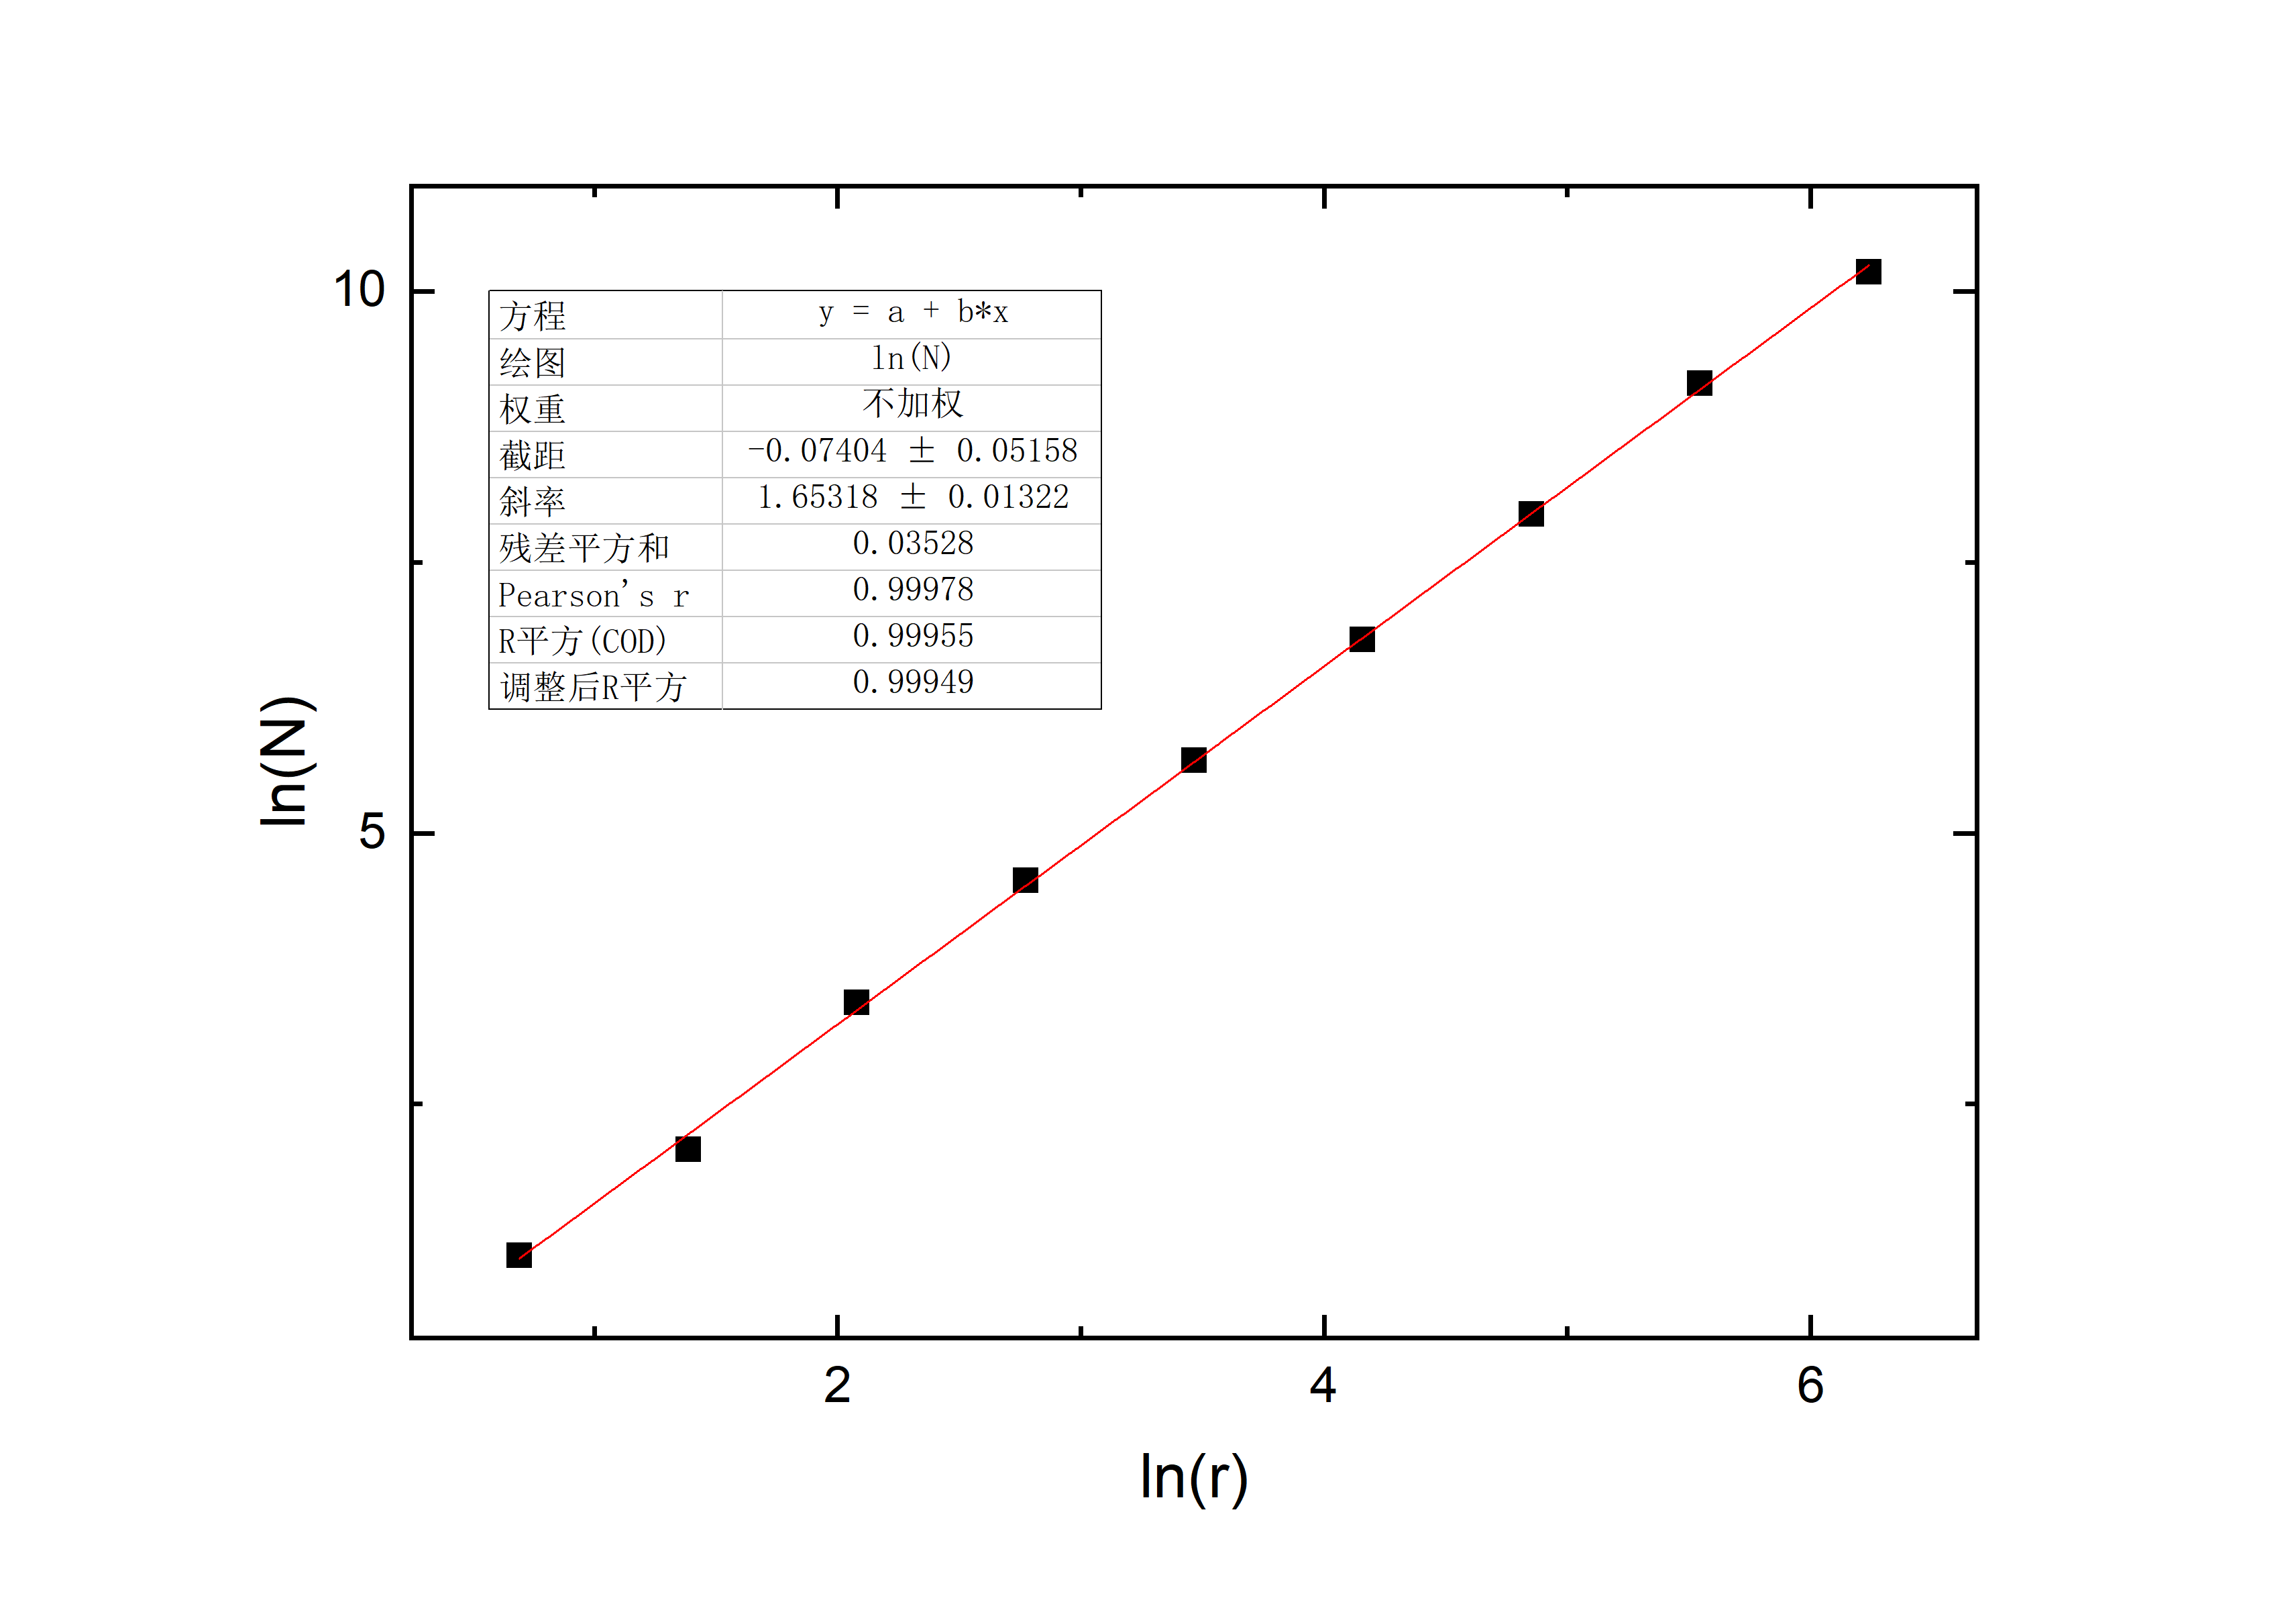
\includegraphics[scale=0.5]{sandbox}
	\captionsetup{font={small},labelfont=bf}
	\caption{\heiti\zihao{-5}Sandbox拟合结果}
	\label{fig:2}
\end{figure}
由图可得拟合结果斜率即分形维数为D=1.65318$ \pm 0.01322 $,与标准结果二维下分形维数结果D=1.65较为接近。
\subsection{面积-回转半径法}
接下来讨论面积-回转半径法取粒子数等于$ N=2-2^{15} $下,拟合结果如图\ref*{fig:3}
		\begin{figure}[!h]
	
	\centering
	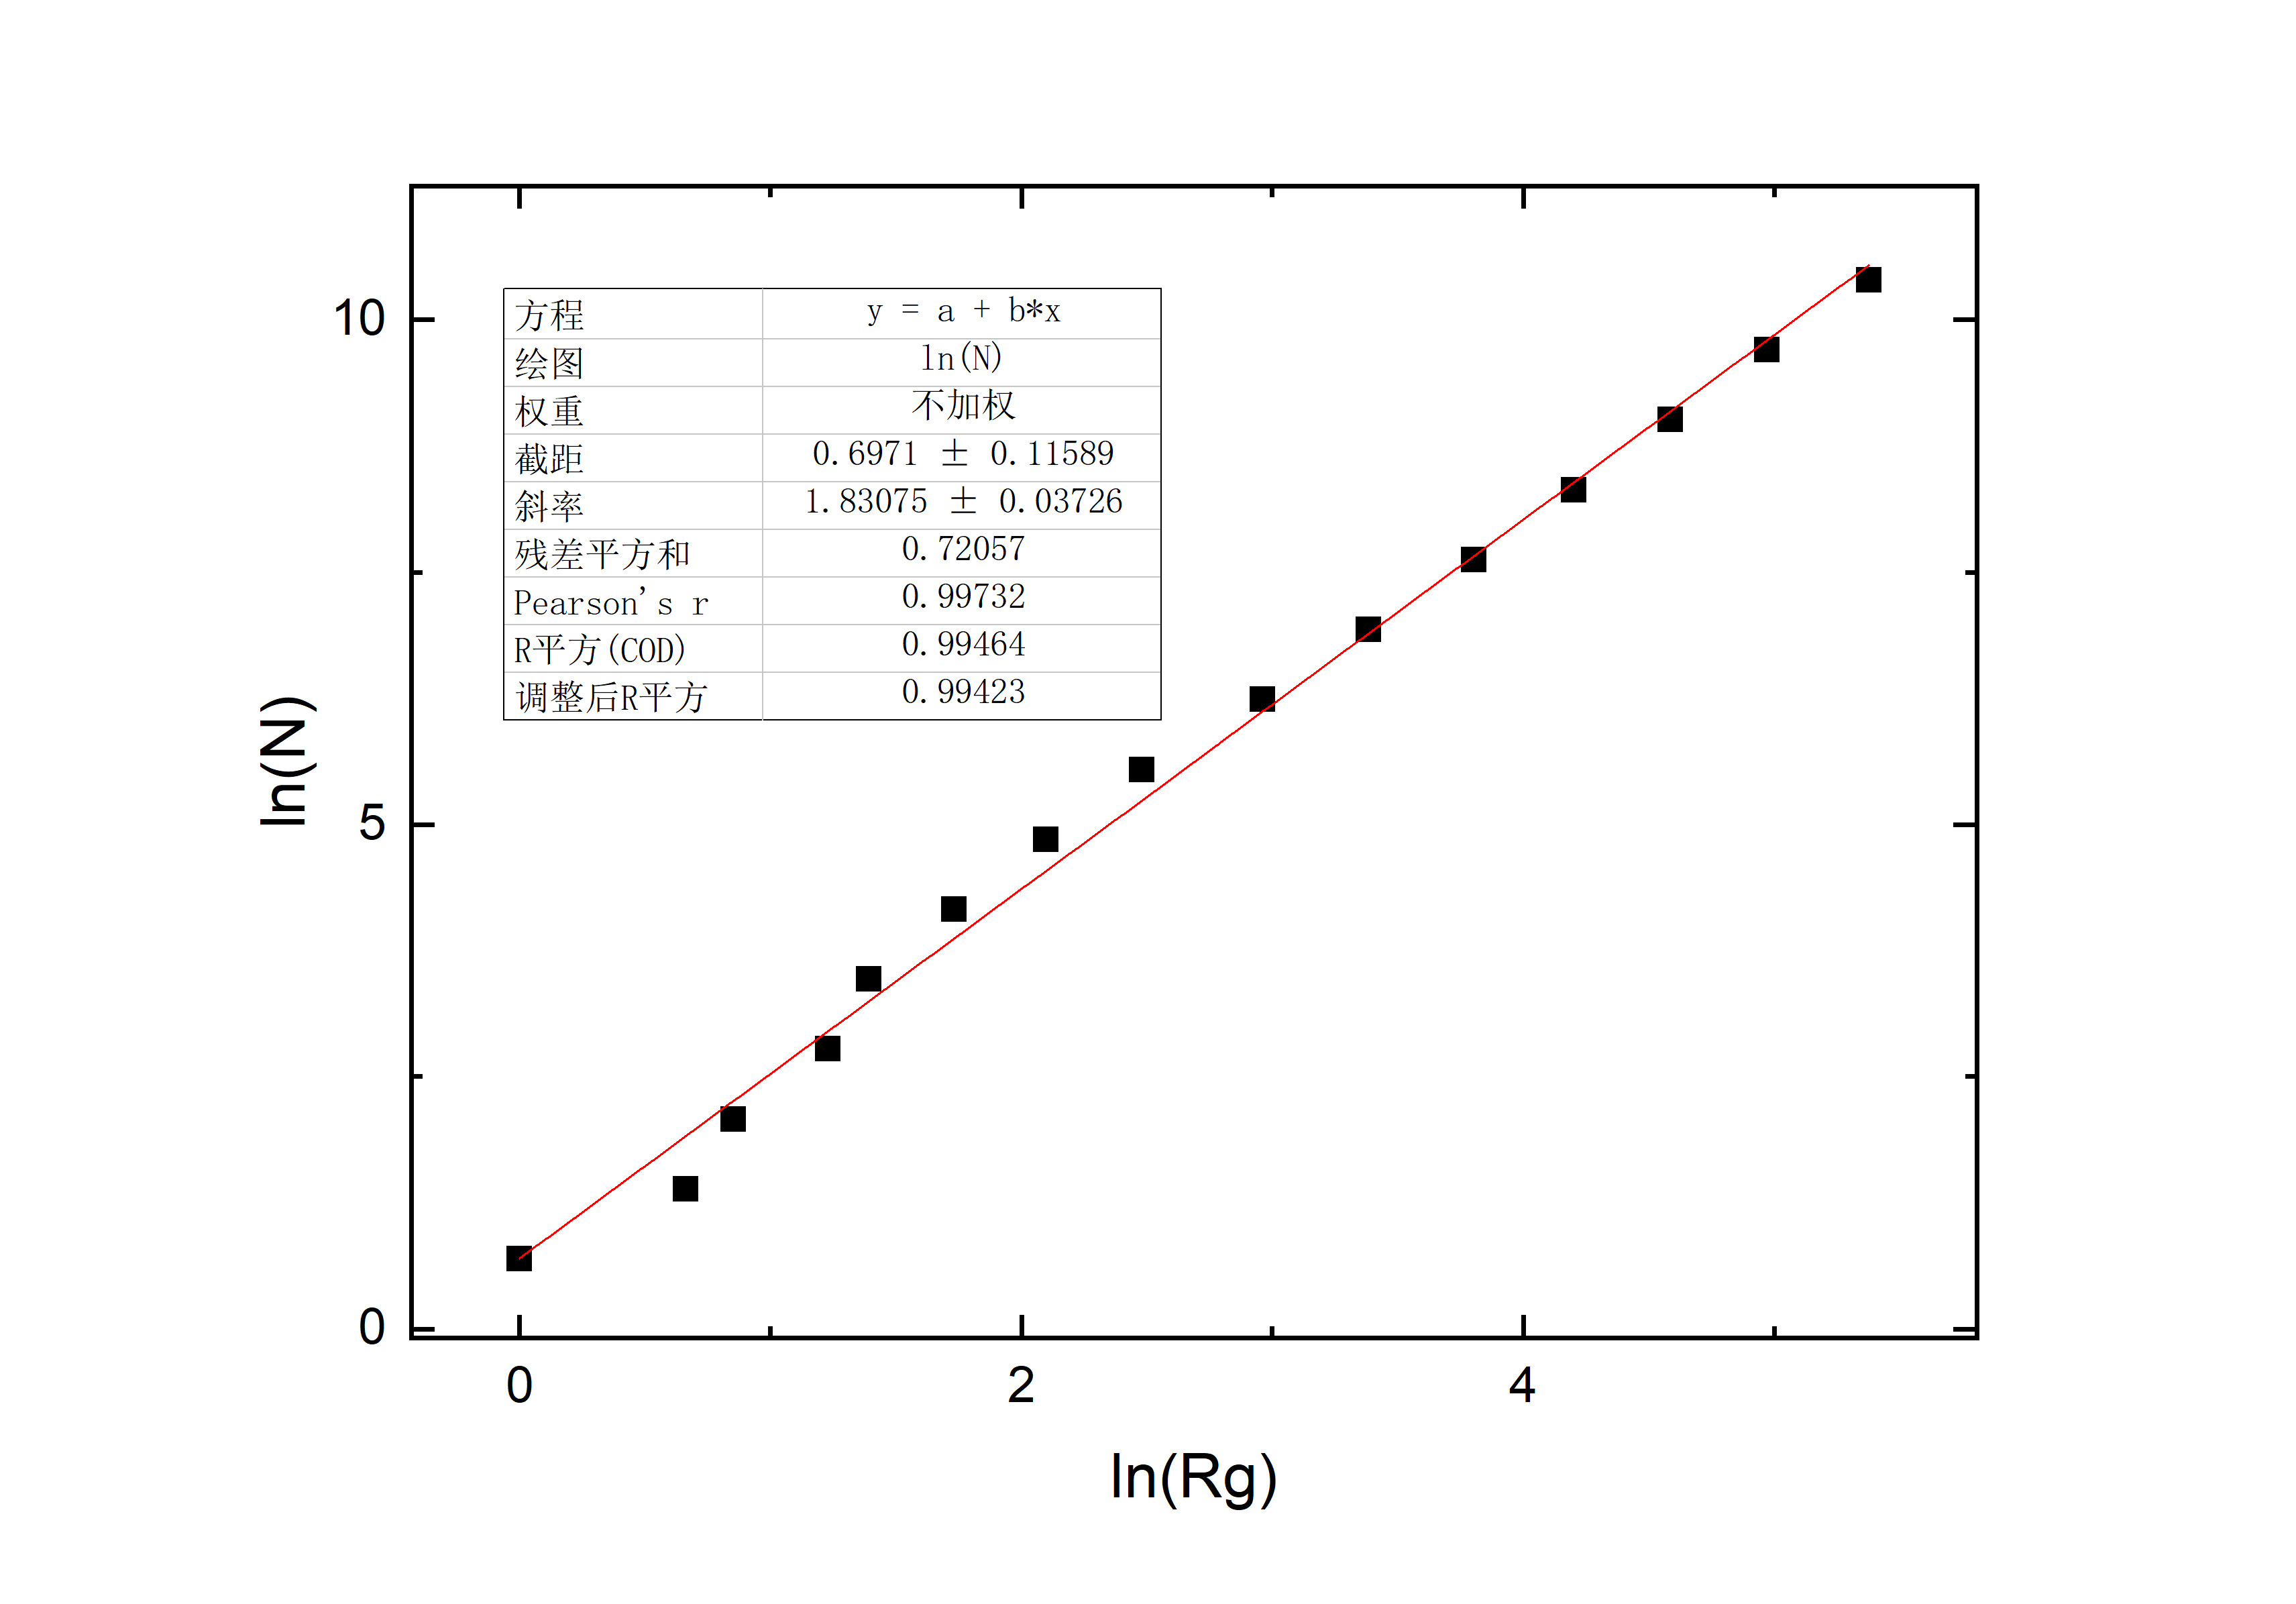
\includegraphics[scale=0.5]{Rg}
	\captionsetup{font={small},labelfont=bf}
	\caption{\heiti\zihao{-5}面积-回转半径法拟合结果}
	\label{fig:3}
\end{figure}
可见结果D=$ 1.83075\pm 0.03726 $, 与标准结果相差较大。由于在开始阶段点数较少的情况下误差较大,可以将开始的点舍弃,得到的结果为
		\begin{figure}[!h]
	
	\centering
	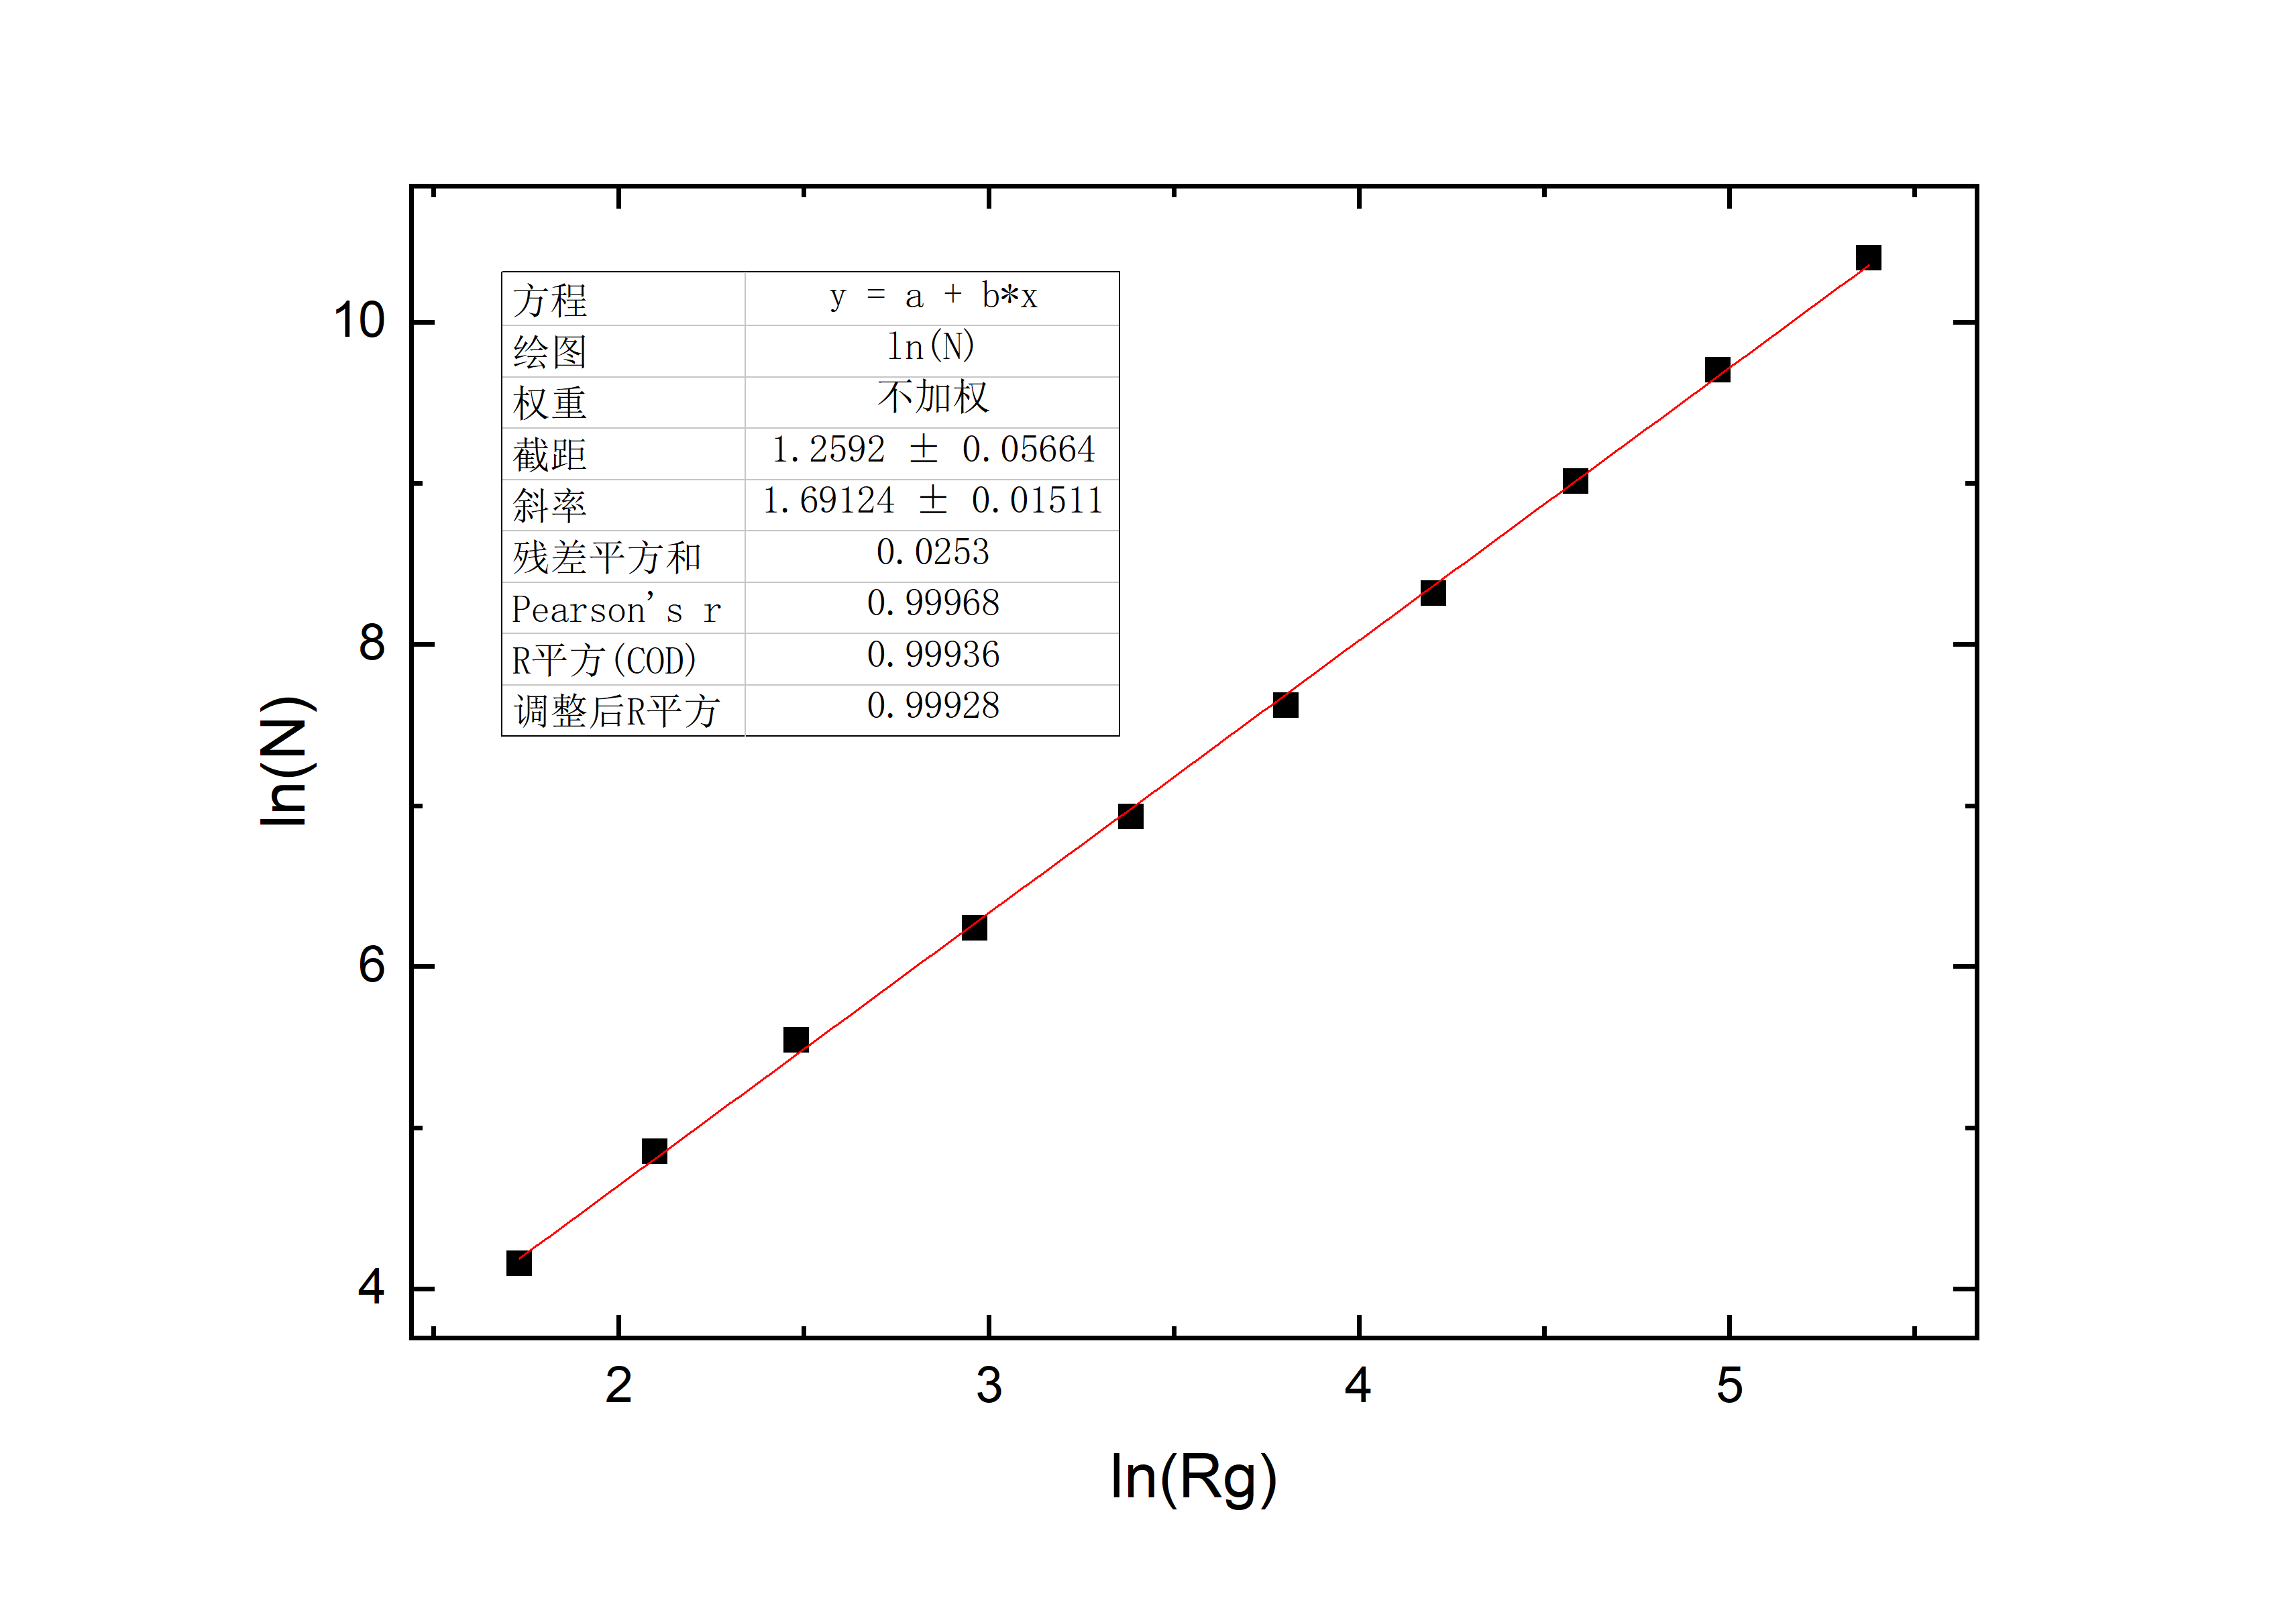
\includegraphics[scale=0.5]{Rg_1}
	\captionsetup{font={small},labelfont=bf}
	\caption{\heiti\zihao{-5}面积-回转半径法舍去初始点拟合结果}
	\label{fig:4}
\end{figure}
可见结果D=$ 1.69124\pm 0.01511 $,结果更接近标准结果,拟合也更接近线性。
	\section{结论}
	根据模拟的结果,可以得到对于中心单核生长的DLA,Sandbox计数法的结果更加准确,适合单中心生长的分形维数计算。而面积-回旋半径计数法的误差相对更大,可能是由于这里推广模型,将同一平面上的多个生长推广为同一中心生长的不同时间段,导致结果的偶然性更大,实际分形是受之间时间的生长情况影响的,而平面上多个核生长则是相对独立的结果进行平均,因此该方法有较大的误差。
\end{document}